% XCircuit output "krivka_vyp_t012.tex" for LaTeX input from krivka_vyp_t012.ps
\def\putbox#1#2#3#4{\makebox[0in][l]{\makebox[#1][l]{}\raisebox{\baselineskip}[0in][0in]{\raisebox{#2}[0in][0in]{\scalebox{#3}{#4}}}}}
\def\rightbox#1{\makebox[0in][r]{#1}}
\def\centbox#1{\makebox[0in]{#1}}
\def\topbox#1{\raisebox{-0.60\baselineskip}[0in][0in]{#1}}
\def\midbox#1{\raisebox{-0.20\baselineskip}[0in][0in]{#1}}
   \scalebox{0.8}{
   \normalsize
   \parbox{2.35417in}{
   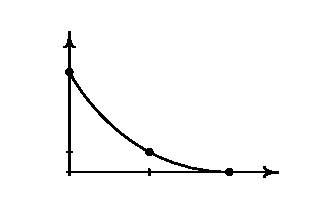
\includegraphics[scale=1.25]{krivka_vyp_t012}\\
   % translate x=-9 y=147 scale 0.30
   \putbox{0.06in}{1.34in}{1.20}{$g(t)$}%
   \putbox{2.11in}{0.09in}{1.20}{$t$}%
   \putbox{1.69in}{0.09in}{1.20}{$t_2$}%
   \putbox{1.02in}{0.09in}{1.20}{$t_1$}%
   \putbox{0.36in}{0.09in}{1.20}{$t_0$}%
   \putbox{0.15in}{0.21in}{1.20}{$G_2$}%
   \putbox{0.15in}{0.38in}{1.20}{$G_1$}%
   \putbox{0.15in}{1.04in}{1.20}{$G_0$}%
   } % close 'parbox'
   } % close 'scalebox'
   \vspace{-\baselineskip} % this is not necessary, but looks better
